\chapter*{Introduction}
\addcontentsline{toc}{chapter}{Introduction}

Speaking of programming languages, the present world of web development is divided into several nearly disjoint communities. Each of these communities focuses primarily on different aspect of development, for instance security, reliability or simplicity. However, the emphasized aspect of development is merely a consequence of the actual programming language selected for the implementation. Speaking of programming languages, we implicitly mean the server-side programming languages as the thesis is focuses mainly on them.

When it comes down to numbers, PHP: Hypertext Preprocessor (PHP) is the ultimate winner with the percentual usage between the websites surveyed of 60 to 70 \%. The second place holds ASP.NET with 10\% - 20\% usage. The third and fourth places are occupied by Java and Ruby, both situated around the border of 5 \% of usage \citep{w3techs.surveys, builwith.survey}. 

Previous statistics show that if we were to sum the websites implemented in PHP and .NET, we would end up with almost 80 \% of all surveyed, and presumably 8 out of 10 all existing, web applications. Moreover, unifying the two technologies would benefit both communities. Where the PHP community could make use of security and manageability advantages of pre-compiled code, the .NET developers will be given means to use dynamic features of the PHP language and a vast of community libraries. This is the ultimate goal of Peachpie, a modern PHP to .NET compiler, that is currently in development.

Many web oriented PHP frameworks have been developed by utilizing built-in functionalities of PHP such as response and request handling, and providing them in a more abstract way. This results in making the process of web application deployment faster and thus less expensive. Due to lack of any reliable statistics on the PHP web frameworks' usage, custom survey on the topic was performed. Considered parameters were Stack Overflow Trends, Google Trends, GitHub stars, Twitter followers and Facebook likes. This gives us quite accurate information about the popularity of selected frameworks compared to each other, which should at least correspond to their actual usage. Gathered data are displayed in the Figure 1 and apply to 15/04/2020. When evaluated, Wordpress is an absolute winner, followed by Laravel and Shopify that share the second place. Third place holds Symfony and after that comes the rest of compared frameworks such as CodeIgniter, PrestaShop, Zend or CakePHP.

Unfortunately, every web framework wraps PHP in its own unique way and provides special additional features. Some provide a basic functionality in a set of default scripts and a vast library of downloadable components with additional functionalities. Others deliver almost a working solution out of the box and leave the user only with the need to configure content and possibility to install whole features in a form of modules, such frameworks are usually called Content Management Systems or simply CMS. Therefore, each framework requires special treatment during its compilation, making their automatic compilation impossible. The Peachpie developers have successfully compiled Wordpress framework. Shopify is not open-source and thus its source code is not simply accessible. On the other hand, Laravel is open-source, and the same goes for Symfony. Even though Laravel is in popularity superior to Symfony, Symfony is almost twice as old and its packages are produced mostly by teams recognized by the Symfony developers themselves, for example FOS or KnpLabs can be named. Its long lasting stability and guaranteed quality of its packages has proved Symfony to be the perfect adept for compilation.

This work therefore examines the possibilities of compiling the Symfony framework into the .NET platform. However, the Peachpie compiler provides just the tools for a single PHP project into .NET compilation. This approach is unfortunate for the Symfony framework as its philosophy lays in minimal start-up project, where every secondary functionality is provided via additional libraries. Therefore, for the purpose of saving user's compilation and start-up time, those libraries are to be precompiled and supplied to projects in the quantity that they require, rather than to compile the project and all of its libraries for each project over and over again. For this task, The NuGet package manager has been selected as it shares the same ideology with Composer, a package manager that is tightly coupled with the Symfony framework. The ideology mentioned focuses mainly on package and dependency management at the project level. Besides, its wide spread of usage, Visual Studio integration ability and fairly easy usability were also taken into consideration.

\begin{figure}[h]
  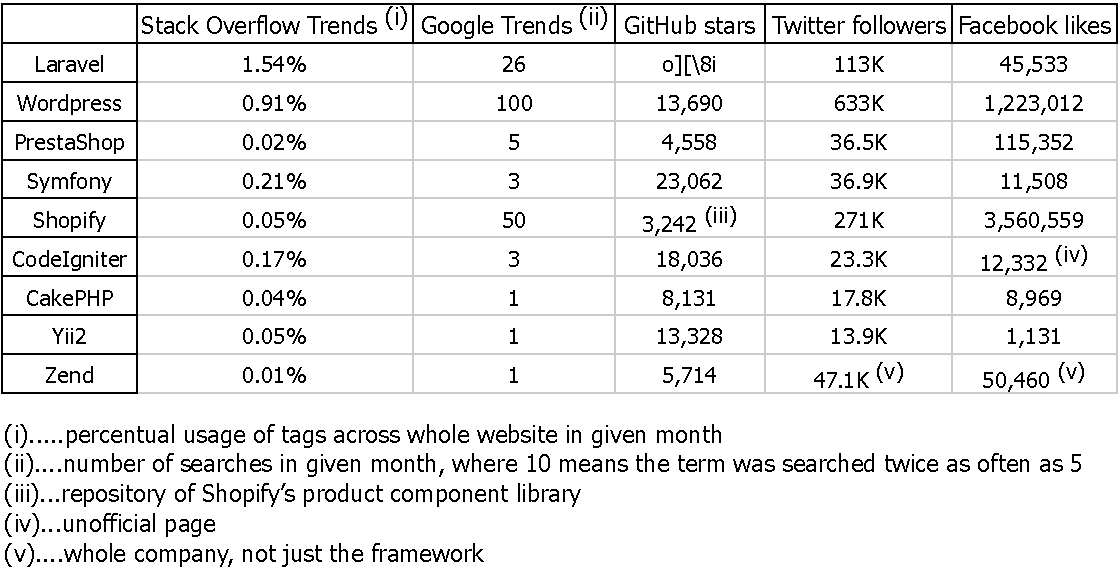
\includegraphics[width=\linewidth]{img/PHP_frameworks_popularity.pdf}
  \caption{PHP frameworks popularity comparison}
  \label{fig:php_frameworks_popularity}
\end{figure}


\section*{Thesis overview}
\addcontentsline{toc}{section}{An overview of the thesis}

The first chapter introduces the PHP programming language along with the tools like the Composer package manager, the Symfony framework and Twig template engine. The second chapter provides general overview of the C\# programming language and tools associated with it: NuGet package manager, ASP.NET Core and Razor template engine. Chapter 3 addresses the problematique of compiling one language to another in general and introduces Peachpie, the PHP to .NET compiler. The problem the thesis aims to resolve along with proposed solution and possible alternatives is introduced in Chapter 4. The fifth chapter focuses on the Symfony Components compilation and the tools that assist the process. The way Symfony projects are compiled and deployed is discussed in Chapter 6. Chapter 7 describes actual usage of the toolkit provided with two exemplar applications.
